% Part B study guide: Fronthaul Load Management for B5G Wireless Communications
% Build: latexmk -pdf PartB_study_guide.tex
\documentclass[11pt,a4paper]{article}
\usepackage[margin=2.1cm]{geometry}
\usepackage[T1]{fontenc}
\usepackage{lmodern}
\usepackage{microtype}
\usepackage{amsmath,amssymb}
\usepackage{booktabs,longtable,array,tabularx}
\usepackage[table,dvipsnames]{xcolor}
\usepackage{enumitem}
\usepackage{graphicx}
\usepackage[most]{tcolorbox}
\usepackage{tikz}
\usetikzlibrary{arrows.meta,positioning,fit,decorations.pathreplacing,calc}
\usepackage{titlesec}
\usepackage{fancyhdr}
\usepackage[colorlinks=true,linkcolor=iitblue,urlcolor=iitblue]{hyperref}

\definecolor{iitblue}{RGB}{16,52,110}
\definecolor{accent}{RGB}{200,40,40}
\definecolor{good}{RGB}{20,120,60}
\definecolor{gold}{RGB}{214,160,30}
\definecolor{soft}{RGB}{238,242,250}

\graphicspath{{../report/figures/}{../results/fhlm/figures/}}

\newcommand{\rstar}{r^\star}
\setlength{\parindent}{0pt}
\setlength{\parskip}{5pt}
\setlist{itemsep=2pt,topsep=3pt}

\titleformat{\section}{\Large\bfseries\color{iitblue}}{\thesection}{0.6em}{}[\vspace{-2pt}{\color{iitblue}\titlerule[0.8pt]}]
\titleformat{\subsection}{\large\bfseries\color{iitblue!85!black}}{\thesubsection}{0.5em}{}

\pagestyle{fancy}
\fancyhf{}
\lhead{\small\color{gray}Part B study guide}
\rhead{\small\color{gray}Fronthaul Load Management for B5G}
\cfoot{\small\thepage}
\renewcommand{\headrulewidth}{0.3pt}

\newtcolorbox{idea}[1][]{enhanced,colback=soft,colframe=iitblue,boxrule=0.7pt,arc=2pt,left=6pt,right=6pt,top=4pt,bottom=4pt,fonttitle=\bfseries,title={#1}}
\newtcolorbox{plain}[1][]{enhanced,colback=good!6,colframe=good!70!black,boxrule=0.6pt,arc=2pt,left=6pt,right=6pt,top=4pt,bottom=4pt,fonttitle=\bfseries,title={#1}}
\newtcolorbox{warn}[1][]{enhanced,colback=accent!5,colframe=accent!80!black,boxrule=0.6pt,arc=2pt,left=6pt,right=6pt,top=4pt,bottom=4pt,fonttitle=\bfseries,title={#1}}
\newtcolorbox{say}{enhanced,colback=gold!10,colframe=gold!80!black,boxrule=0.6pt,arc=2pt,left=6pt,right=6pt,top=4pt,bottom=4pt,fonttitle=\bfseries,title={How to say it in the viva}}

\newcounter{qn}
\newcommand{\Q}[1]{\refstepcounter{qn}\par\medskip\noindent{\color{iitblue}\textbf{Q\theqn.\ #1}}\par\nopagebreak}
\newcommand{\A}{\noindent\textbf{A.}\ }

\begin{document}

% ---------------------------------------------------------------------
\begin{titlepage}
\centering
\vspace*{2.5cm}
{\color{iitblue}\rule{\linewidth}{1.2pt}}\\[10pt]
{\Huge\bfseries\color{iitblue} Part B, from scratch}\\[8pt]
{\Large Sharing one fronthaul link between many cells}\\[6pt]
{\large A study guide with every term explained and a viva question bank}\\[10pt]
{\color{iitblue}\rule{\linewidth}{1.2pt}}\\[1.5cm]
{\large B.Tech.\ Project: \emph{Fronthaul Load Management for B5G Wireless Communications}}\\[6pt]
Harshvardhan Choudhary (230002027) \quad Mayank Yadav (230002041)\\[3pt]
Guide: Dr.\ Sumit Gautam \quad Department of Electrical Engineering, IIT Indore\\[2cm]
\begin{minipage}{0.82\linewidth}
\begin{idea}[How to use this guide]
Read Sections 1--4 in order once: they build the whole story from zero, one idea at a time. Sections 5--7 give the evidence (how we tested and what we found). Section 8 is an A--Z glossary of every term; look things up there whenever a word is unclear. Section 9 is a bank of questions professors are likely to ask, each with a short model answer. Section 10 is a one-page cheat sheet of the numbers to remember.

All numbers are from the final report (Chapters 5 and 6, plus the appendix proofs).
\end{idea}
\end{minipage}
\vfill
\end{titlepage}

\tableofcontents
\newpage

% =====================================================================
\section{The story in plain words}
% =====================================================================

\subsection{What problem are we solving?}

When you use your phone, the radio signal goes to an antenna on a tower. From there it must travel to a computer that decodes it. In modern 5G networks built to the \textbf{Open RAN (O-RAN)} standard, this work is split between two boxes:
\begin{itemize}
  \item the \textbf{radio unit (RU)} on the mast, which holds the antennas and does the first, simple signal processing;
  \item the \textbf{distributed unit (DU)}, a server a few kilometres away, which does the heavy processing (channel estimation, decoding) and runs the \textbf{scheduler} that decides which user transmits on which frequencies.
\end{itemize}
The cable between them is the \textbf{fronthaul}. It carries digitised radio samples (\textbf{IQ samples}), so it is very fast (gigabits per second) and very strict about delay: a sample that arrives late is useless.

To save money, operators do not give every cell its own fronthaul cable all the way to the DU. Many cells connect to one \textbf{aggregation switch}, and one shared Ethernet link (in our case 25\,Gbit/s, written \textbf{25GE}) carries all their traffic to the DU pool. The link is deliberately \textbf{smaller than the sum of all cells' peak rates}, because cells rarely peak at the same time. This trick is called \textbf{statistical multiplexing}, and running a link below the total peak is \textbf{over-subscription}.

\begin{plain}[The one-sentence problem]
Most of the time the shared link is big enough. But when bursts from several cells happen together, it is not, and somebody's data must wait or be dropped. \textbf{Part B decides, in advance, how much of the link each cell may use, so that the least important data is the data that gets lost.}
\end{plain}

\subsection{Why is this hard?}

Three facts make it hard:
\begin{enumerate}
  \item \textbf{Different cells have different deadlines.} 3 of our 8 cells are \textbf{low-latency (LL)} cells (think of factory robots, AR/VR, gaming): their bits must be delivered within \textbf{2\,ms}, and they matter more (priority weight 3). The other 5 are \textbf{eMBB} cells (enhanced mobile broadband: video, browsing, downloads) with a \textbf{10\,ms} deadline and weight 1.
  \item \textbf{We must decide before we see the traffic.} The controller cannot change the split every 0.5\,ms slot. Real O-RAN control loops (the \textbf{near-RT RIC}) run every 10\,ms or slower. So every 10\,ms we fix a \textbf{budget} (a maximum number of bits per slot) for each cell and keep it fixed for the next 20 slots.
  \item \textbf{Our information is old.} The measurements we decide on (the \textbf{telemetry}) are already 1\,ms old when they arrive.
\end{enumerate}
So the controller has to guess the future traffic of each cell for the next $\approx$11\,ms, and divide a fixed link between them. If it gives too little to a cell, that cell's bits wait in a queue and, past their deadline, are \textbf{dropped} (a \textbf{deadline violation}). If it gives too much, capacity sits unused while other cells starve.

\subsection{What did we do? (the four steps)}

\begin{center}
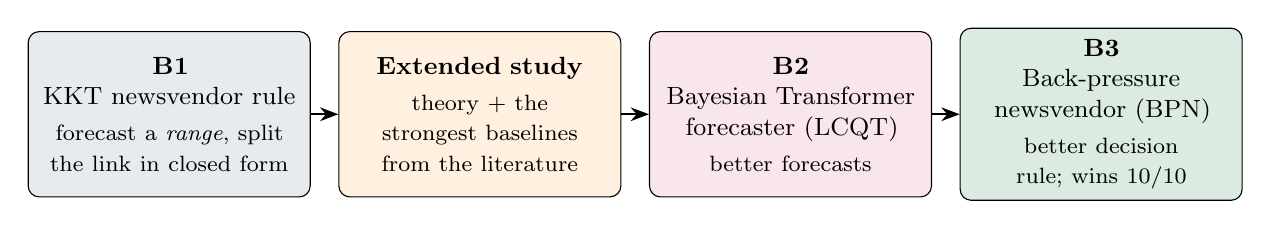
\begin{tikzpicture}[font=\small,>=Stealth,
   s/.style={draw,rounded corners,align=center,text width=3.3cm,minimum height=2.1cm,inner sep=4pt}]
  \node[s,fill=iitblue!10] (b1) {\textbf{B1}\\KKT newsvendor rule\\[2pt]\footnotesize forecast a \emph{range}, split the link in closed form};
  \node[s,fill=orange!12,right=0.35cm of b1] (ext) {\textbf{Extended study}\\[2pt]\footnotesize theory + the strongest baselines from the literature};
  \node[s,fill=purple!10,right=0.35cm of ext] (b2) {\textbf{B2}\\Bayesian Transformer forecaster (LCQT)\\[2pt]\footnotesize better forecasts};
  \node[s,fill=good!15,right=0.35cm of b2] (b3) {\textbf{B3}\\Back-pressure newsvendor (BPN)\\[2pt]\footnotesize better decision rule; wins 10/10};
  \draw[->,thick] (b1) -- (ext); \draw[->,thick] (ext) -- (b2); \draw[->,thick] (b2) -- (b3);
\end{tikzpicture}
\end{center}

\begin{enumerate}
  \item \textbf{B1.} Instead of predicting one number for each cell's future need, predict a \emph{range} (several \textbf{quantiles}). Then split the link with a formula that comes from optimisation theory (the \textbf{KKT conditions}) applied to a classic inventory problem (the \textbf{newsvendor problem}). Result: best of 12 controllers on every scenario of two traffic families.
  \item \textbf{Extended study.} We wrote the problem down formally (a \textbf{POMDP}), derived bounds on the quantity we forecast, added a third traffic family, and implemented the two strongest controllers we could find in the literature: \textbf{predictive MaxWeight} and a policy learned by the \textbf{cross-entropy method (CEM)}. These beat B1 in 9 of 10 scenarios, which told us where B1 is weak.
  \item \textbf{B2.} We built a better forecaster: a small Transformer neural network designed for this link (\textbf{LCQT}), with Bayesian uncertainty. It improves B1 on every seed, but only by 1.4\,\% at high load. Lesson: the remaining gap is not the forecast, it is the \emph{decision rule}.
  \item \textbf{B3.} We designed a new decision rule, the \textbf{back-pressure newsvendor (BPN)}, which contains both strongest baselines as special cases and adds what they lack. It beats the best baseline in \textbf{all 10 scenarios of all 3 traffic families}, by 3--25\,\%.
\end{enumerate}

\begin{say}
``Part A makes each cell's fronthaul smaller. Part B decides how a shared, over-subscribed link is divided between cells with different deadlines, every 10 milliseconds, before the traffic is seen. We forecast each cell's deadline-feasible rate as a range and split the link with a closed-form newsvendor rule; our final controller, the back-pressure newsvendor, beats the strongest baselines from queueing theory and policy search in all ten scenarios of three traffic families.''
\end{say}

% =====================================================================
\section{The setup, in numbers}
% =====================================================================

\subsection{Basic radio units of time and frequency}

\begin{itemize}
  \item \textbf{Slot}: the basic scheduling time unit of 5G. With 30\,kHz subcarrier spacing a slot is \textbf{0.5\,ms} and contains \textbf{14 OFDM symbols}.
  \item \textbf{PRB (physical resource block)}: the basic frequency unit, \textbf{12 subcarriers} wide. A 100\,MHz carrier has \textbf{273 PRBs}.
  \item \textbf{Layer}: one MIMO spatial stream. Our cells use up to \textbf{4 layers}.
  \item \textbf{PRB-layer}: one PRB on one layer in one slot. In the O-RAN 7-2x fronthaul, \emph{the load is the number of scheduled PRB-layers}, not the number of user bits.
\end{itemize}

\subsection{How many bits one PRB-layer costs on the fronthaul}

The 7-2x fronthaul compresses IQ samples with \textbf{block floating point (BFP)}: each I and Q value is sent as a $b$-bit mantissa, and the 12 subcarriers of one PRB share one exponent byte. Per PRB-layer per slot:
\[
  \beta(b) = (\underbrace{12\cdot 2\cdot b}_{\text{I and Q of 12 subcarriers}} + \underbrace{8}_{\text{exponent byte}})\cdot \underbrace{14}_{\text{symbols}}\cdot \underbrace{\kappa}_{\text{packet overhead }1.08}, \qquad \beta(9) = 3387\text{ bits}.
\]
6-bit, 12-bit and 14-bit mantissas scale this by 0.68, 1.32 and 1.54. \textbf{This is exactly where Part A enters Part B}: compression changes $\beta$ and therefore the load on the link.

A cell that must deliver $a_i(t)$ user bits with spectral efficiency $\eta_i(t)$ (user bits per PRB-layer, set by the channel quality) needs $\lceil a_i/\eta_i\rceil$ PRB-layers, so its fronthaul demand is
\[ d_i(t) = \lceil a_i(t)/\eta_i(t)\rceil\,\beta . \]
Two cells with the same user traffic but different channel quality can differ by 2--3$\times$ in fronthaul load.

\subsection{The scenario}

\begin{center}
\renewcommand{\arraystretch}{1.15}
\begin{tabular}{ll}
\toprule
Quantity & Value and meaning \\
\midrule
Cells $N$ & 8: 3 LL (deadline $D = 2$\,ms, weight $w = 3$), 5 eMBB ($D = 10$\,ms, $w = 1$) \\
Link & 25GE; 3\,\% reserved for control, management and sync planes \\
Capacity $C$ & $25\text{ Gbit/s}\times 0.97\times 0.5\text{ ms} = \mathbf{12.125}$ \textbf{Mbit per slot} \\
Per-cell peak & $273 \times 4 \times 3387 \approx 3.7$ Mbit per slot $\approx 7.4$ Gbit/s \\
Over-subscription & sum of the 8 peaks $= 2.44\,C$ \\
Control interval $T$ & 20 slots = 10\,ms (budgets held fixed for this long) \\
Telemetry delay $\tau$ & 2 slots = 1\,ms \\
Lead time $H$ & $H = T + \tau = 22$ slots that the decision must cover without seeing them \\
Cap of cell $i$ & $\mathrm{cap}_i = 273\,L_i\,\beta$ (its maximum possible demand) \\
\bottomrule
\end{tabular}
\end{center}

\subsection{What happens every 10\,ms (the control loop)}

\begin{center}
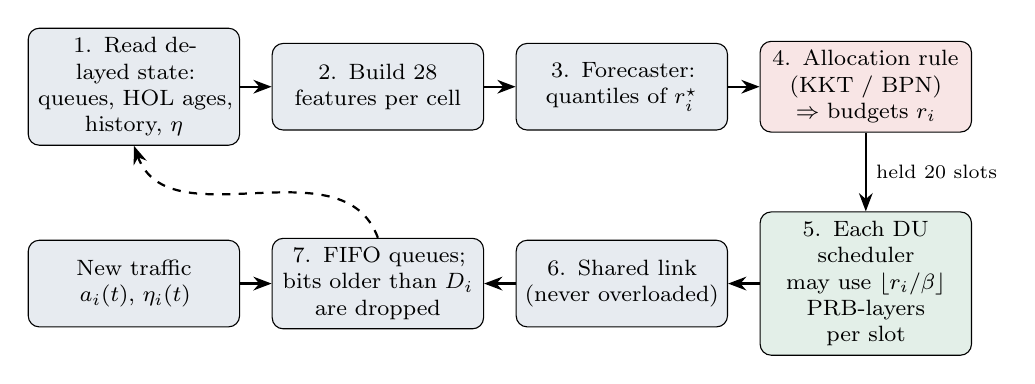
\begin{tikzpicture}[font=\footnotesize,>=Stealth,node distance=0.45cm and 0.4cm,
   st/.style={draw,rounded corners,fill=iitblue!10,align=center,minimum height=1.1cm,text width=2.45cm}]
  \node[st] (obs) {1. Read delayed state:\\queues, HOL ages,\\history, $\eta$};
  \node[st,right=of obs] (feat) {2. Build 28\\features per cell};
  \node[st,right=of feat] (gbm) {3. Forecaster:\\quantiles of $\rstar_i$};
  \node[st,right=of gbm,fill=accent!12] (kkt) {4. Allocation rule\\(KKT / BPN)\\$\Rightarrow$ budgets $r_i$};
  \node[st,below=1.0cm of kkt,fill=good!12] (du) {5. Each DU scheduler\\may use $\lfloor r_i/\beta\rfloor$\\PRB-layers per slot};
  \node[st,left=of du] (link) {6. Shared link\\(never overloaded)};
  \node[st,left=of link] (q) {7. FIFO queues;\\bits older than $D_i$\\are dropped};
  \node[st,left=of q] (traffic) {New traffic\\$a_i(t)$, $\eta_i(t)$};
  \draw[->,thick] (obs) -- (feat); \draw[->,thick] (feat) -- (gbm); \draw[->,thick] (gbm) -- (kkt);
  \draw[->,thick] (kkt) -- node[right,font=\scriptsize]{held 20 slots} (du);
  \draw[->,thick] (du) -- (link); \draw[->,thick] (link) -- (q); \draw[->,thick] (traffic) -- (q);
  \draw[->,thick,dashed] (q.north) to[out=110,in=-70] (obs.south);
\end{tikzpicture}
\end{center}

Because the budgets always add up to at most $C$, the link itself never overflows. Congestion shows up instead as bits waiting in each cell's queue at the DU, and bits that wait longer than their deadline are dropped.

\subsection{The score: weighted violation ratio $V_w$}

\[
  V_w = \frac{\sum_i w_i\cdot(\text{bits of cell } i \text{ that missed their deadline})}{\sum_i w_i\cdot(\text{bits of cell } i \text{ that arrived})}.
\]
It is the fraction of traffic lost, where an LL bit counts 3 times and an eMBB bit once. \textbf{Lower is better.} It was fixed \emph{before} any tuning, so we could not choose the metric that flatters us. We also report: per-class violations, link utilisation, unused allocation, DU delay, Jain fairness and decision time.

% =====================================================================
\section{The core ideas, one at a time}
% =====================================================================

\subsection{Idea 1: forecast the deadline-feasible rate $\rstar$, not the traffic volume}

What should we forecast? The obvious answer is ``how many bits will arrive''. That is wrong for deadline traffic: a 2\,ms cell with a short burst needs much more than its average rate, because the burst must be cleared within 2\,ms.

\begin{idea}[Definition: deadline-feasible rate]
For arrivals $a_1,\dots,a_H$ over the horizon and a deadline of $D$ slots,
\[
  \rstar(a,D) = \max_{1\le s\le e\le H}\ \frac{\sum_{t=s}^{e} a_t}{\,e - s + 1 + D\,}.
\]
It is \textbf{the smallest constant rate at which no bit misses its deadline}.
\end{idea}

\textbf{Why this formula?} Take any window of slots from $s$ to $e$. All the bits that arrive in this window must leave before the last one's deadline, i.e.\ within $e - s + 1 + D$ slots. So a constant rate $r$ is enough only if $r \ge (\text{bits in window})/(\text{window length} + D)$ for \emph{every} window. The largest of these ratios is $\rstar$. In network-calculus language, this is the \textbf{service-curve condition}. We verified in tests that it is tight to one PRB-layer.

\textbf{Worked example.} One burst of 8 units arrives in a single slot, nothing else.
\begin{itemize}
  \item Deadline $D = 1$ slot: best window is the burst slot alone: $\rstar = 8/(1+1) = 4$.
  \item Deadline $D = 7$ slots: $\rstar = 8/(1+7) = 1$.
\end{itemize}
A short deadline forces a rate close to the peak, while a long deadline lets you smooth the burst down to the mean. For our 2\,ms cells, $\rstar$ is typically 2--3$\times$ the mean rate and strongly \textbf{right-skewed} (usually moderate, occasionally very large).

\textbf{What every deadline-aware controller needs.}
\[
  \text{need}_i = B_i + \rstar_i, \qquad B_i = \frac{\text{backlog}_i}{\text{slack}_i}.
\]
$B_i$ is the rate needed to clear what is \emph{already queued} before its deadline (backlog divided by the remaining time, the \textbf{slack}); $\rstar_i$ covers what has \emph{not yet arrived}. $B_i$ is known; $\rstar_i$ is uncertain. Controllers differ only in (1) how they estimate $\rstar_i$ and (2) how they split a shortage when the needs add up to more than $C$.

\subsection{Idea 2: forecast a range (quantiles), not one number}

Because $\rstar$ is skewed, one predicted number (for example the median) is a poor basis for reserving capacity: half the time the true value is higher, and for an LL cell that means drops. So we predict a \textbf{distribution}, described by six \textbf{quantiles}:
\[ \alpha \in \{0.05,\ 0.25,\ 0.5,\ 0.75,\ 0.9,\ 0.95\}. \]
The $\alpha$-quantile $q_\alpha$ is the value that the true $\rstar$ stays below with probability $\alpha$. For example, $q_{0.9}$ is a value that is exceeded only 10\,\% of the time.

\textbf{The B1 forecaster.} One \textbf{gradient-boosted tree} model per quantile level (scikit-learn histogram GBM, 300 trees, 15 leaves), trained with the \textbf{pinball loss}, on 101k rows from 16 training traces. Training takes 12\,s on a CPU.

\textbf{Target.} $y_i = \rstar(d_i[t-\tau : t+T],\,D_i)/\mathrm{cap}_i$, the coming horizon's $\rstar$ divided by the cell's peak, so all cells are on the same 0--1 scale.

\textbf{The 28 features} use only past slots (no peeking into the future): the last six horizon means and their mean, standard deviation and maximum; two exponentially weighted averages; the last four slot demands; $\rstar$ of the last three horizons; the relative spectral efficiency; $D_i/H$; and a one-hot cell identifier.

\textbf{Calibration.} On validation data the quantiles cover 5.6 / 25.6 / 50.7 / 75.3 / 89.9 / 94.9\,\% at nominal 5 / 25 / 50 / 75 / 90 / 95\,\%: calibrated within about one percentage point. Pinball loss 0.0224, versus 0.0293 for a simple window median.

\subsection{Idea 3: split the link with the KKT newsvendor rule}

\textbf{The newsvendor analogy.} A newspaper seller must decide in the morning how many papers to stock, before knowing demand. Too few: lost sales. Too many: waste. The optimal stock is a \emph{quantile} of the demand distribution. Our problem is the same: each budget is ``stock'' chosen before demand is known. The twist is that all cells share one link, so it is a \textbf{constrained, multi-item newsvendor}.

\textbf{The optimisation problem.} Choose budgets to maximise the expected priority-weighted need that gets served:
\[
  \max_{r}\ \sum_i w_i\,\mathbb{E}\big[\min(B_i + \rstar_i,\ r_i)\big]
  \quad\text{s.t.}\quad \sum_i r_i \le C,\quad 0\le r_i\le \mathrm{cap}_i .
\]
$\min(\text{need}, \text{budget})$ is the part of the need that the budget covers. The objective is a sum of separate per-cell terms (\textbf{separable}), and each term is \textbf{concave}: each extra bit of budget is worth a little less than the previous one. Its derivative is
\[
  \frac{\partial}{\partial r_i} = w_i\,\big(1 - F_i(r_i - B_i)\big)
  = w_i \times \Pr(\text{this marginal bit of budget is actually needed}),
\]
where $F_i$ is the forecast distribution (cumulative distribution function, CDF) of $\rstar_i$.

\textbf{The solution (KKT).} For a concave, separable problem with linear constraints, the \textbf{Karush--Kuhn--Tucker (KKT) conditions} are necessary and sufficient, so they give the \emph{global} optimum. Setting the marginal value equal to one common price $\lambda$ and inverting:
\begin{idea}[The KKT newsvendor rule]
\[
  r_i(\lambda) = \mathrm{clip}\Big(B_i + F_i^{-1}\big(1 - \lambda/w_i\big),\ 0,\ \mathrm{cap}_i\Big)
\]
$\lambda \ge 0$ is the \textbf{shadow price} of link capacity. It is found by \textbf{bisection} (60 halving steps) so that $\sum_i r_i(\lambda) = C$. If the link is not full, $\lambda = 0$ and every cell gets its full predicted support. $F_i^{-1}$ (the \textbf{quantile function}) is interpolated linearly between the six forecast quantiles. Cost: a few tens of microseconds for 8 cells, under 0.1\,ms.
\end{idea}

\textbf{Interpretation.} Every cell first gets its backlog rate $B_i$, then a quantile of its forecast. The quantile level $1 - \lambda/w_i$ is \emph{higher for higher-priority cells}. At the optimum every cell is cut at the \textbf{same priority-weighted risk}: $w_i\Pr(\text{need}_i > r_i) = \lambda$. A cell with a wide (uncertain) forecast automatically receives more margin; a cell with a confident forecast receives about its median. \textbf{The margins are derived, not tuned.}

\textbf{Toy example 1 (from the slides).} Bisection returns $\lambda = 0.6$. An LL cell ($w = 3$) is funded to its $1 - 0.6/3 = 0.8$ quantile; an eMBB cell ($w = 1$) to its $1 - 0.6 = 0.4$ quantile.

\textbf{Toy example 2 (worked bisection).} $C = 10$. LL cell: $B = 2$, $w = 3$, $\rstar$ uniform on $[0,6]$ so $F^{-1}(p) = 6p$. eMBB cell: $B = 1$, $w = 1$, $\rstar$ uniform on $[0,8]$ so $F^{-1}(p) = 8p$. For $\lambda < 1$:
\[
  r_{\rm LL} = 2 + 6(1 - \lambda/3),\quad r_{\rm eMBB} = 1 + 8(1-\lambda),\quad
  \sum = 17 - 10\lambda = 10 \Rightarrow \lambda = 0.7 .
\]
So $r_{\rm LL} = 6.6$ (its 0.767 quantile) and $r_{\rm eMBB} = 3.4$ (its 0.3 quantile). Check: weighted tail risk is $3\times(1-0.767) = 0.7$ for LL and $1\times(1-0.3) = 0.7$ for eMBB: equal, as promised.

\subsection{The four proven properties (appendix of the report)}

\begin{description}[leftmargin=0.5cm,style=nextline]
  \item[P1 Feasibility] For any forecast and any $\lambda$, every budget is between 0 and its cap, and the bisection output satisfies $\sum_i r_i \le C$: \emph{the link is never overloaded}. (Each $r_i(\lambda)$ decreases with $\lambda$; bisection keeps the invariant ``sum at the upper end $\le C$''.)
  \item[P2 Equal weighted tail probability] At an interior optimum $w_i(1 - F_i(r_i - B_i)) = \lambda$ for every cell. With point forecasts (no uncertainty) the rule reduces to filling cells in priority order.
  \item[P3 Backlog first] Any cell with $\lambda < w_i$ gets at least its backlog rate $\min(B_i,\mathrm{cap}_i)$ before the \emph{uncertain} demand of any equal- or lower-priority cell is funded. Known, queued bits are protected first.
  \item[P4 Robustness to miscalibration] If the forecast CDF $F_i$ is at most $\epsilon$ away from the true CDF $G_i$ everywhere, the loss in the objective is at most $2\,\epsilon\,w_{\max}\,C$: it grows \emph{at most linearly} in the forecast error. A slightly wrong forecast cannot cause a disaster.
\end{description}

% =====================================================================
\section{All the controllers, explained}
% =====================================================================

A \textbf{controller} (also called a \emph{policy} or \emph{allocation rule}) is the algorithm that, every 10\,ms, looks at the delayed state and outputs the 8 budgets $r_i$. Every controller sees exactly the same traffic and the same stale observations; all were tuned on validation seeds; all redistribute unused capacity and use the same weights and backlog rate.

\subsection{The 12 controllers of B1 (NCC comparison)}

\begin{center}
\small
\renewcommand{\arraystretch}{1.2}
\begin{tabularx}{\linewidth}{>{\raggedright\arraybackslash}p{3.6cm}X}
\toprule
Controller & What it does, in plain words \\
\midrule
Static equal share & Every cell gets $C/8$, always. Ignores traffic. Worst baseline; shows how bad doing nothing is. \\
Reactive proportional & Measures each cell's recent average rate (an EWMA) and splits the link in proportion. Reacts to the past; does not know about deadlines. \\
MaxWeight & Classic queueing rule: serve cells in order of priority $\times$ queue length, with an urgency term for the age of the oldest bit (HOL age). Throughput-optimal in theory, but myopic and deadline-unaware. \\
Deadline-aware reactive & Uses the \emph{last observed} $\rstar$ as the forecast of the next one, then a deadline-weighted water-fill. ``Tomorrow will look like today.'' \\
Point forecast (GBM median) & \textbf{Key ablation.} Same GBM model as ours, but uses only one number, the median, with a deadline-weighted water-fill. Tests whether the \emph{range} matters. \\
Fixed global quantile (0.75) & Same GBM, but every cell reserves the same quantile level (tuned: 0.75). Tests whether ``just reserve a high quantile'' is the trick. It is not. \\
Proposed, window quantiles (no ML) & Our KKT rule, but the quantiles are just the empirical quantiles of the last 30 horizons. Tests whether the rule works without machine learning. \\
\textbf{Proposed (GBM + KKT)} & \textbf{Our B1 method.} GBM quantiles of $\rstar$ + KKT newsvendor split. \\
Oracle water-fill & Knows the \emph{true future} $\rstar$ and water-fills. Not implementable; shown as a reference for how good a controller could be. \\
Oracle + KKT & True future $\rstar$ fed to the KKT rule. Also a reference only. \\
\bottomrule
\end{tabularx}
\end{center}

(The report counts 12 reference controllers in the B1 comparison; the table lists the main ones. Margins of $\{0, 0.25, 0.5\}$, EWMA windows and persistence windows were tuned for every baseline on validation seeds. A margin of 0 was best for all of them.)

\subsection{The extended study adds 7 more (19 in total)}

\begin{description}[leftmargin=0.5cm,style=nextline]
  \item[Predictive MaxWeight (Huang et al.)] A \emph{Lyapunov-drift} controller. Each cell's pressure is $\pi_i = w_i(Q_i + \ell H m_i)$: its queue plus what its forecast median $m_i$ says will arrive. Cells are served in order of pressure, each up to $Q_i/T + (1+\mu)m_i$. Very good on short bursts. One of the two \textbf{strongest baselines}.
  \item[CEM class-level policy] A 3-parameter policy: each LL cell reserves $B_i + F_i^{-1}(p_{\rm LL})$, each eMBB cell $B_i + F_i^{-1}(p_{\rm eMBB})$, and a shortage is shared by weighted water-filling with a learned LL weight $w_{\rm LL}$. The three numbers are learned by the \textbf{cross-entropy method} (CEM) on training seeds. It is a small, reliable stand-in for a deep reinforcement-learning xApp. The other \textbf{strongest baseline}.
  \item[Markov-chain KKT] Fits a Markov chain to each cell's traffic online and computes the distribution of $\rstar$ from it, with no training data. Within 3--9\,\% of the learned rule.
  \item[Bound-quantile KKT] Uses the theoretical Chernoff bound as the forecast. Valid but very conservative.
  \item[Tuned-weight KKT] The KKT rule with the LL weight re-tuned. Gains only 1--4\,\% (explained in Section 6.6).
\end{description}

\subsection{Words used to describe allocation styles}

\begin{itemize}
  \item \textbf{Water-filling}: pour capacity into cells like water into containers of different depths until the total equals $C$; each cell gets $\min(\text{level}, \text{its need})$ for a common level.
  \item \textbf{Reservation}: each cell gets a protected amount (e.g.\ a high quantile) whether or not it uses it. Protects LL cells but wastes capacity when the reserved amount is not used.
  \item \textbf{Back-pressure}: serve whoever has the biggest queue pressure first. Wastes less, but ignores deadlines and uncertainty.
\end{itemize}

% =====================================================================
\section{How we tested it (evaluation protocol)}
% =====================================================================

\subsection{Three traffic families}

We used three independent traffic models so that no conclusion depends on one model.
\begin{description}[leftmargin=0.5cm,style=nextline]
  \item[Family S (synthetic, bursty)] Gamma-distributed background traffic plus \textbf{ON/OFF bursts} whose ON and OFF durations follow heavy-tailed \textbf{Pareto} distributions ($\alpha_{\rm on} = 1.5$, $\alpha_{\rm off} = 1.8$), slow load regimes and spectral-efficiency drift. Five scenarios: low (offered load 0.50), moderate (0.65), high (0.80), flash crowds, and a \textbf{held-out shift} (a traffic distribution never seen in training or tuning).
  \item[Family G (3GPP, standards-based)] Nothing hand-designed: 3GPP TR 38.901 \textbf{UMa} (urban macro) geometry with 7 interfering sites, \textbf{Jakes fading}, the TS 38.214 \textbf{CQI} table, \textbf{FTP Model 3} traffic for eMBB and \textbf{XR video} at 60\,fps for LL cells. Demand is the output of a round-robin PRB scheduler. Scenarios: moderate (0.65), high (0.80).
  \item[Family M (Markov-modulated)] Gamma sources whose rate switches between idle, normal and burst phases following a Markov chain. Scenarios: moderate, high, and a \textbf{semi-Markov} held-out shift with Pareto sojourns.
\end{description}
That gives \textbf{10 scenarios} in total (5 S + 2 G + 3 M).

\textbf{Offered load} is the average demand divided by the link capacity; 0.80 means that on average 80\,\% of the link is needed, but bursts push it far above 100\,\%.

\subsection{Seeds, splits and statistics}

\begin{itemize}
  \item A \textbf{seed} is the starting number of the random generator; one seed = one reproducible traffic trace. Train seeds 1000--1015, validation 2000--2003, test 3000--3019. They never overlap, and every forecaster is \textbf{frozen} before testing, so there is no \textbf{data leakage}.
  \item Each scenario: \textbf{20 test seeds $\times$ 20{,}000 slots} (10\,s each), after a 1{,}000-slot \textbf{warm-up} (so queues start in a realistic state).
  \item All controllers see \textbf{identical traces}, so we can compare them \textbf{paired}: on the same seed, did A beat B? Seed-to-seed variation is dominated by burst timing, which all controllers share, so paired tests are much more sensitive than comparing averages.
  \item We report: mean relative change of $V_w$ with a \textbf{95\,\% bootstrap confidence interval}, the number of seeds won out of 20, and a \textbf{Wilcoxon signed-rank test} with \textbf{Holm correction} for multiple comparisons.
\end{itemize}

% =====================================================================
\section{What we found (results)}
% =====================================================================

\subsection{B1 main result (Family S)}

\begin{center}
\small
\begin{tabular}{lccccc}
\toprule
$V_w$ [\%], 20 seeds & low 0.50 & mod.\ 0.65 & high 0.80 & flash & shift \\
\midrule
Static equal share & 4.45 & 9.65 & 15.46 & 19.15 & 22.31 \\
Reactive proportional & 0.83 & 4.11 & 9.20 & 12.27 & 11.70 \\
MaxWeight & 0.90 & 4.85 & 11.54 & 15.24 & 12.31 \\
Deadline-aware reactive & 0.52 & 4.24 & 11.03 & 14.51 & 12.56 \\
Point forecast (GBM median) & 0.27 & 3.23 & 9.70 & 13.33 & 11.30 \\
Fixed global quantile (0.75) & 0.34 & 4.35 & 11.76 & 15.09 & 12.85 \\
Window quantiles (no ML) & 0.25 & 2.57 & 8.72 & 12.67 & 10.22 \\
\rowcolor{good!12}\textbf{Proposed (GBM + KKT)} & \textbf{0.15} & \textbf{2.15} & \textbf{8.00} & \textbf{11.76} & \textbf{10.04} \\
\color{gray}Oracle water-fill & \color{gray}0.07 & \color{gray}1.62 & \color{gray}6.89 & \color{gray}10.16 & \color{gray}6.69 \\
\bottomrule
\end{tabular}
\end{center}

Paired, per seed: the proposed rule beats the point forecast by 11--43\,\%, the fixed quantile by 22--54\,\%, deadline-aware reactive by 19--70\,\% and MaxWeight by 18--83\,\%, on \textbf{20/20 seeds in every scenario}, $p < 0.01$. Weakest case: only $-4\,\%$ against reactive proportional under flash crowds (16/20 seeds), because reactive proportional starves LL cells but serves eMBB better.

\subsection{Where the gain comes from}

At high load, among deadline-aware controllers, the proposed rule has the lowest eMBB violation (12.3\,\%), the highest utilisation (72.2\,\%) and the best Jain fairness (0.997). It adds margin only where the forecast is wide. One global quantile over-protects LL and wastes about a third of its allocation. In time-series plots the reactive controller is \emph{one interval late} at every burst, while the proposed rule raises the budget at burst onset, when the forecast range widens.

\subsection{Ablations (what carries the gain)}

\begin{enumerate}
  \item \textbf{Range vs.\ one number} (same model): $-11$ to $-43\,\%$, 20/20 seeds everywhere. Representing uncertainty matters.
  \item \textbf{Per-cell KKT level vs.\ one global level} (same forecast): $-22$ to $-54\,\%$. The level must be set per cell by the link constraint.
  \item \textbf{GBM vs.\ window (no-ML) quantiles} under the same rule: GBM adds $-7$ to $-37\,\%$. But even the no-ML version beats the point forecast everywhere, so \textbf{the rule carries the method}; ML adds on top.
\end{enumerate}

\subsection{Family G (3GPP traffic)}

The result reproduces on traffic we did not design: best implementable controller at both loads, 20/20 seeds. At high load: 8.01\,\% vs 8.98 (point forecast), 11.53 (deadline-aware), 15.94 (reactive). Also best under the \emph{unweighted} ratio (14.4\,\%). A forecaster trained only on Family S and transferred without retraining still beats every reactive controller.

\subsection{Robustness and operating range}

\begin{itemize}
  \item \textbf{Miscalibration} (P4 in practice): shift every quantile level by $\epsilon$. Under-reserving ($\epsilon < 0$) is almost harmless because a common shift is absorbed by $\lambda$. Even at $\epsilon = +0.3$ the rule (9.45\,\%) still matches the point forecast (9.46\,\%).
  \item \textbf{Control interval $T$}: best controller at every $T$ from 2 to 10\,ms (the near-RT RIC range). At $T = 2$\,ms (3.07\,\%) it even beats the oracle water-fill. At $T = 20$\,ms it loses to reactive proportional.
  \item \textbf{Telemetry delay $\tau$}: advantage over reactive is $-16\,\%$ at $\tau = 0$, shrinking to $-2\,\%$ at $\tau = 5$\,ms. Fresher data helps a forecaster more.
  \item \textbf{Priority weight}: raising the LL weight from 3 to 5 lowers our $V_w$ from 8.00 to 6.93\,\%, while reactive proportional rises from 9.20 to 10.56\,\%. The more the operator values LL, the bigger our advantage.
  \item \textbf{Decision time}: the KKT rule $<0.1$\,ms; whole controller incl.\ features and $6\times300$ trees: 3.5\,ms in Python, inside the 10\,ms interval. Our vectorised numpy tree traversal is 6.7$\times$ faster than scikit-learn's \texttt{predict}.
\end{itemize}

\subsection{Part A $\times$ Part B}

Same user traffic; only the BFP mantissa width changes $\beta$:
\begin{center}
\begin{tabular}{lcccc}
\toprule
BFP width & offered load & Reactive prop. & Point forecast & \textbf{Proposed} \\
\midrule
6 bit & 0.44 & 0.22 & 0.15 & \textbf{0.11} \\
9 bit & 0.65 & 3.90 & 3.00 & \textbf{1.96} \\
\bottomrule
\end{tabular}
\end{center}
\textbf{Compression sets the regime; allocation decides the loss inside it.} At 0.65 load the rule halves reactive control's loss. Near full load no split can help, and Part A must bring the load down.

\subsection{Extended study: the honest twist}

With the \emph{same} GBM forecaster, CEM is best in 6/10 scenarios and predictive MaxWeight in 3/10 (all on bursty Family S); B1 wins none of the 10 against them. Diagnosis of $\lambda$: at high load the link is binding in 99.8--100\,\% of epochs and $\lambda^\ast \ge w_{\rm eMBB}$ in 50--58\,\% of them. That means in half the epochs every eMBB cell is already at its lowest quantile, so re-tuning the LL weight gains only 1--4\,\%. \textbf{The gap is structural, not a constant}: CEM gains from decoupled per-class levels and a different sharing rule; back-pressure gains from not wasting reserved capacity.

\textbf{Theory results.} We wrote the problem as a POMDP (intractable: hundreds of continuous state dimensions, unknown traffic law, actions held for $T$ slots) and implemented the three main approximation families: one-step stochastic programs (KKT), Lyapunov drift (predictive MaxWeight), direct policy search (CEM). For Markov traffic we derived the effective bandwidth, a Chernoff--union bound on $\Pr(\rstar > x)$, a large-deadline decay rate, and a pathwise \textbf{shortfall sandwich} $(D+1)(\rstar - r)^+ \le V(r) \le \sum_t(a_t - r)^+$ (violated volume at constant rate $r$). The bounds are valid in all runs but 25--100$\times$ too conservative at 2--10\,ms deadlines, a strong argument for \emph{learning} the distribution instead of computing it from a model.

% =====================================================================
\section{B2 and B3 in depth}
% =====================================================================

\subsection{B2: LCQT, a Bayesian link-aware quantile Transformer}

A drop-in replacement for the GBM forecaster. It is built from known components (PatchTST, iTransformer, TFT, FiLM, deep ensembles, MC dropout) plus \textbf{six modifications for the shared link}:
\begin{enumerate}
  \item \textbf{Deadline-aware patch tokens.} 352 slots of history are cut into 16 \emph{patches} of 22 slots ($= H$). Each patch token carries its own $\rstar$ at the cell's deadline, plus its mean and maximum. A summary token holds the 28 GBM features.
  \item \textbf{Deadline/priority FiLM.} One network serves both LL and eMBB cells; its internal features are scaled and shifted by a small network of $(D_i/H, p_i)$.
  \item \textbf{Link-aware cross-cell attention.} After the per-cell temporal encoder (2 layers, width 48, 4 heads), attention runs \emph{across the 8 cells} that share the link, so each cell's forecast can use the others' state.
  \item \textbf{Non-crossing quantile head.} $q_k = q_{k-1} + \mathrm{softplus}(a_k)$, so $q_{0.05}\le q_{0.25}\le\dots$ is guaranteed.
  \item \textbf{Bayesian mixture layer.} 3 independently trained models $\times$ 8 MC-dropout passes = 24 posterior samples. The KKT rule receives their \emph{mixture} $\hat F_i(x) = \frac{1}{24}\sum_s F_i^{(s)}(x)$, \emph{not} the average of their quantiles. If the samples disagree, the mixture is wider, so an uncertain cell gets more margin at the same price.
  \item \textbf{Differentiable KKT layer.} Lets the network be trained through the allocation. Forward: bisection finds $\lambda^\ast$. Backward: the \textbf{implicit function theorem} on the binding constraint $g(\lambda,q) = \sum_i r_i - C = 0$ gives $\partial\lambda^\ast/\partial q = -(\partial g/\partial q)/(\partial g/\partial\lambda)$. Matches the numpy allocator to $10^{-6}$.
\end{enumerate}
63k parameters; about 6 minutes of CPU training (40 epochs, AdamW with one-cycle schedule, early stopping on validation pinball loss).

\textbf{Results.} Pinball loss $-4.5\,\%$ (0.0214 vs 0.0224), 90\,\% interval width $-8\,\%$ with higher coverage. The Bayesian mixture is the best-calibrated model (90\,\% coverage 0.919 in distribution, 0.808 under shift). In closed loop with the KKT rule, paired against GBM + KKT: $-20.8\,\%$ (low), $-6.1\,\%$ (moderate), $-1.4\,\%$ (high), on 20/20 seeds each.

\textbf{Decision-focused variant (DF-LCQT)} trained directly on the shortfall-sandwich lower bound of dropped bits (plus a pinball regulariser), with one DAgger round. It was \emph{not} better than the plain Bayesian LCQT: 7.93 vs 7.89\,\% at high load.

\textbf{Lesson.} With the best forecaster we could build, the KKT rule improves only modestly at high load, while CEM and predictive MaxWeight remain 14--28\,\% lower. \textbf{The gap is the decision structure, not the forecast.} That motivated B3.

\subsection{B3: the back-pressure newsvendor (BPN)}

\textbf{Diagnosis.} A budget is a \emph{per-cell cap}. Capacity reserved for an LL cell's upper quantile and then not used is lost to everyone else. So pure reservation (KKT) protects LL but leaves eMBB short (12.3\,\% eMBB violation, 72.2\,\% utilisation). Back-pressure wastes less but ignores deadlines and uncertainty.

\textbf{Idea.} \emph{Fill a base in back-pressure order, then spend the leftover on newsvendor margins.}

\textbf{Stage 1 (base).}
\begin{itemize}
  \item Base rate $b_i = a\,Q_i/T + (1-a)\,B_i$: a mix of MaxWeight's queue drain rate ($Q_i/T$) and the deadline-aware backlog rate ($B_i$).
  \item Base demand $d_i = b_i + (1+\mu)\,\hat F_i^{-1}(p^0_{c(i)})$: plus a class-specific base quantile $p^0$ of the forecast.
  \item If base demands exceed the link, the shortage is shared in proportion to $v_c(\pi_i/\bar\pi)^{\eta}$, with pressure $\pi_i = Q_i + \ell H m_i$ (queue plus look-ahead times forecast median).
  \item The exponent $\eta$ slides continuously from \textbf{reservation} ($\eta = 0$, class-weighted water-fill) to \textbf{strict back-pressure order} ($\eta = \eta_{\max}$).
\end{itemize}
\textbf{Stage 2 (leftover by KKT).} $r_i = \max\big(r_i^{(1)},\ b_i + \hat F_i^{-1}(1 - \lambda/\omega_{c(i)})\big)$, with $\lambda$ by bisection so that $\sum_i r_i = C$: newsvendor margins only where the forecast is wide.

\textbf{Both strongest baselines are special cases} (verified exactly by unit tests):
\begin{itemize}
  \item predictive MaxWeight: $a = 1$, $p^0 = 0.5$, $\mu$ = its margin, $\eta = \eta_{\max}$;
  \item CEM class-level policy: $a = 0$, $p^0$ = its class levels, $v_{\rm LL} = w_{\rm LL}$, $\eta = 0$.
\end{itemize}
So a search started from each baseline's tuned optimum can only match or improve on both.

\textbf{Learning, with equal effort.} 8 parameters $\theta = (a,\mu,p^0_{\rm LL},p^0_{\rm eMBB},v_{\rm LL},\eta,\ell,\omega_{\rm LL})$ learned by CEM on \emph{training} seeds only (8 episodes per candidate), started from both baselines' optima. For fairness, \textbf{both baselines were re-tuned with the same CEM search}. BPN v1 has 6 parameters and a stage 1 that is always strict back-pressure; BPN v2 adds $\eta$ and $\mu$ and so also contains reservation.

\textbf{Results.}
\begin{itemize}
  \item S high: BPN 5.23\,\% vs 5.98 (CEM-tuned predictive MaxWeight) and 6.58 (re-searched CEM); within 6--10\,\% of the oracle-informed KKT rule. Highest utilisation (76.1\,\%, even above the oracle-informed KKT's 74.8\,\%) and lowest eMBB violation (4.8--4.9\,\%).
  \item With the Bayesian LCQT forecaster: 5.05\,\% at S high, 8.34\,\% flash, 8.92\,\% shift, the best results of the whole project. The B2 forecaster pays off more with a better decision rule.
  \item \textbf{BPN v2 beats the best baseline in all 10 scenarios} (best baseline = better of predictive MaxWeight and CEM, separately per scenario, each in its best tuning) by 3.4--25.3\,\%, 20/20 seeds in 8 scenarios, 19/20 at G high, 15/20 at S low; all $p \le 0.024$ after Holm correction.
  \item v1 loses on Family G because it cannot represent reservation, which long 3GPP bursts (FTP files, XR frames) need. v2 contains it and generalises.
\end{itemize}

\textbf{What the policy learned (interpretable).}
\begin{center}
\begin{tabular}{lccc}
\toprule
Family & $\eta$ & $a$ & $(p^0_{\rm LL}, p^0_{\rm eMBB})$ \\
\midrule
S (bursty) & 6: strict back-pressure & 0.98 & (0.41, 0.45) \\
G (3GPP) & 0: reservation & 0.31 & (0.94, 0.73) \\
M (Markov) & 0: reservation & 0.34 & (0.84, 0.31) \\
\bottomrule
\end{tabular}
\end{center}
The search rediscovers the regime map on its own: \textbf{back-pressure for short bursts, reservation for long ones}. BPN is not a black box; it tells the operator which structure suits its traffic. Decision time 2.2--3.5\,ms in Python.

% =====================================================================
\section{Glossary: every term, A to Z}
% =====================================================================

\small
\renewcommand{\arraystretch}{1.25}
\begin{longtable}{>{\raggedright\arraybackslash\bfseries}p{3.6cm}>{\raggedright\arraybackslash}p{12.2cm}}
\toprule
\normalfont\textbf{Term} & \textbf{Meaning} \\
\midrule
\endfirsthead
\toprule
\normalfont\textbf{Term} & \textbf{Meaning} \\
\midrule
\endhead
\bottomrule
\endfoot
\multicolumn{2}{l}{\color{iitblue}\normalsize\textbf{Network and radio}}\\
5G / B5G & Fifth generation of mobile networks / ``beyond 5G'', i.e.\ 5G-Advanced and 6G. \\
RAN & Radio access network: everything between the phone and the core network (antennas, radio units, baseband processing). \\
D-RAN & Distributed RAN: the full baseband unit sits at every tower; only backhaul leaves the site. \\
C-RAN & Centralised RAN: baseband units of many sites pooled in one place; needs a huge constant-rate CPRI fronthaul. \\
O-RAN / Open RAN & An industry standard (O-RAN Alliance) that splits the RAN into units from different vendors with open interfaces. \\
RU / O-RU & Radio unit on the mast: antennas, RF and (in split 7-2x) the low physical layer (FFT, cyclic prefix, optionally precoding). \\
DU / O-DU & Distributed unit: server that runs the high physical layer (channel estimation, equalisation, decoding), the MAC scheduler and RLC. \\
CU / O-CU & Central unit: runs PDCP, RRC, SDAP; can serve many DUs. \\
Fronthaul & Link between RU and DU. Carries IQ samples; tens of Gbit/s; about 100\,$\mu$s latency budget. \textbf{The subject of this project.} \\
Midhaul & Link between DU and CU; carries packets at about the user data rate; a few ms latency. \\
Backhaul & Link between CU and the core network; aggregated traffic; about 10\,ms latency. \\
X-haul & Collective name for fronthaul, midhaul and backhaul. \\
Functional split & Where the protocol stack is cut between central and remote units; 3GPP TR 38.801 defines Options 1--8. \\
Split 7-2x & The O-RAN intra-PHY split. The fronthaul carries frequency-domain IQ only for \emph{scheduled} PRBs, so its load follows the traffic. \\
CPRI / eCPRI & Common Public Radio Interface: the old constant-rate fronthaul protocol / its packet-based (Ethernet) successor used by 7-2x. \\
25GE & 25 Gigabit Ethernet: the shared link of our scenario. \\
C/M/S-plane & Control, management and synchronisation planes of the fronthaul; we reserve 3\,\% of the link for them. (The IQ data is the U-plane, user plane.) \\
Aggregation switch & Ethernet switch where many RUs' links merge into one link towards the DU pool. \\
Statistical multiplexing & Sharing one link between many sources that rarely peak together, so the link can be smaller than the sum of peaks. \\
Over-subscription & Running a link whose capacity is below the sum of peak demands (here sum of peaks $= 2.44\,C$). \\
IQ samples & In-phase and quadrature components: the complex numbers that represent a radio signal digitally. \\
BFP & Block floating point: O-RAN compression; each PRB's 12 subcarriers share one exponent, and each I/Q value is a $b$-bit mantissa. \\
$\beta(b)$ & Fronthaul bits per PRB-layer per slot with $b$-bit BFP; $\beta(9) = 3387$ bits. Links Part A and Part B. \\
$\kappa$ & Packet overhead factor (1.08): headers on top of the IQ payload. \\
OFDM & Orthogonal frequency-division multiplexing: the 5G waveform; data on many narrow subcarriers. \\
Subcarrier & One narrow frequency tone of OFDM (30\,kHz wide here). \\
Slot & 0.5\,ms scheduling unit with 14 OFDM symbols (at 30\,kHz spacing). \\
PRB & Physical resource block: 12 subcarriers $\times$ one slot. A 100\,MHz carrier has 273. \\
Layer & One MIMO spatial stream; up to 4 per cell here. \\
PRB-layer & One PRB on one layer in one slot; the unit of fronthaul load. \\
MIMO & Multiple-input multiple-output: many antennas send several streams on the same frequencies. \\
Spectral efficiency $\eta_i$ & User bits carried per PRB-layer; depends on channel quality. Low $\eta$ $\Rightarrow$ more PRBs for the same bits $\Rightarrow$ more fronthaul load. \\
Scheduler (MAC) & The DU function that decides, every slot, which users get which PRBs. Our budget limits how many PRB-layers it may schedule. \\
eMBB & Enhanced mobile broadband: high-rate, delay-tolerant traffic (video, downloads). Here $D = 10$\,ms, $w = 1$. \\
LL cell & Low-latency cell (URLLC-like: industrial control, XR, gaming). Here $D = 2$\,ms, $w = 3$. \\
URLLC & Ultra-reliable low-latency communication: the 5G service class for strict-deadline traffic. \\
RIC & RAN intelligent controller: O-RAN's programmable control platform. \\
Near-RT RIC & Near-real-time RIC: runs \textbf{xApps} in a 10\,ms--1\,s loop; where our controller would live. \\
Non-RT RIC & Non-real-time RIC inside the SMO: runs \textbf{rApps} above 1\,s; trains models, sets policies. \\
xApp / rApp & Applications running on the near-RT / non-RT RIC. \\
E2 / A1 / O1 / F1 & O-RAN interfaces: RIC$\leftrightarrow$CU/DU (E2), non-RT$\leftrightarrow$near-RT RIC (A1), management (O1), CU$\leftrightarrow$DU (F1). \\
SMO & Service management and orchestration framework of O-RAN. \\
Telemetry & Measurements reported to the controller (queues, ages, demand, spectral efficiency); 1\,ms old here. \\
CQI & Channel quality indicator: what the phone reports about channel quality; mapped to a modulation and coding rate via the TS 38.214 table. \\
UMa & Urban macro: the 3GPP TR 38.901 city scenario with tall base stations. \\
Jakes fading & A classic model of how a channel fluctuates in time due to user movement (Doppler). \\
FTP Model 3 & 3GPP traffic model of file downloads with random arrivals; used for eMBB in Family G. \\
XR traffic & Extended-reality video frames at 60\,fps (3GPP TR 38.838); used for LL cells in Family G. \\
Round-robin scheduler & Serves users in turn; used to turn Family G traffic into PRB demand. \\
\multicolumn{2}{l}{\color{iitblue}\normalsize\textbf{Part B model}}\\
Cell $i$ & One of the 8 radio cells sharing the link. \\
Capacity $C$ & Usable link capacity per slot: 12.125\,Mbit. \\
Budget $r_i$ & Maximum fronthaul bits per slot that cell $i$ may send in the coming interval; the controller's output. \\
Cap$_i$ & Largest useful budget: $273\,L_i\,\beta$. \\
Controller / policy / allocation rule & The algorithm that maps the (delayed) state to the 8 budgets every 10\,ms. \\
Control interval $T$ & How long budgets are held: 20 slots = 10\,ms. \\
Decision epoch $t_k$ & The moment a new decision is made ($t_k = kT$). \\
Telemetry delay $\tau$ & Age of the observations at decision time: 2 slots = 1\,ms. \\
Lead time / horizon $H$ & $H = T + \tau$ = 22 slots that the budget must cover without seeing them. \\
Demand $d_i(t)$ & Fronthaul bits cell $i$ wants to send in slot $t$: $\lceil a_i/\eta_i\rceil\beta$. \\
Arrivals $a_i(t)$ & User bits arriving at cell $i$ in slot $t$. \\
Queue $Q_i$ & Bits waiting at the DU for cell $i$ (FIFO: first in, first out). \\
Backlog & Same as the queued bits. \\
HOL age & Head-of-line age: how long the oldest queued bit has been waiting. \\
Slack & Time left before a queued bit's deadline. \\
Backlog rate $B_i$ & Backlog divided by slack: rate needed to clear what is already queued in time. \\
Deadline $D_i$ & Maximum allowed waiting time: 2\,ms (LL) or 10\,ms (eMBB). \\
Deadline violation & A bit dropped because it waited longer than its deadline. \\
Weight / priority $w_i$ & Importance of a cell's bits in the metric: 3 for LL, 1 for eMBB. \\
$V_w$ & Priority-weighted violation ratio: weighted dropped bits / weighted arrived bits. The primary metric; lower is better. \\
Unweighted violation ratio & Same without weights: all bits count equally. \\
Utilisation & Fraction of link capacity actually used to carry bits. \\
Unused allocation & Budget granted but not used (wasted reservation). \\
Jain fairness & $(\sum x_i)^2/(N\sum x_i^2)$ for per-cell values $x_i$ (e.g.\ the fraction of each cell's traffic served); 1 means perfectly fair. \\
Offered load & Mean demand / capacity (0.50, 0.65, 0.80 in our scenarios). \\
Flash crowd & Scenario where many users suddenly become active together. \\
Held-out shift & A traffic distribution never used in training or tuning; tests generalisation. \\
$\rstar$ (deadline-feasible rate) & Smallest constant rate at which no bit of a horizon misses its deadline; what we forecast. \\
need$_i$ & $B_i + \rstar_i$: what a deadline-aware controller wants to give cell $i$. \\
Service curve & Network-calculus concept: a guaranteed minimum amount of service over any time window; $\rstar$ is the service-curve condition for deadline $D$. \\
Network calculus & A theory of worst-case delays in networks using arrival and service curves. \\
Shortage & When the sum of needs exceeds $C$, so somebody must get less. \\
\multicolumn{2}{l}{\color{iitblue}\normalsize\textbf{Forecasting and machine learning}}\\
Point forecast & A single predicted number (here the median). \\
Quantile $q_\alpha$ & Value that the true quantity stays below with probability $\alpha$. \\
Quantile function $F^{-1}$ & Inverse CDF: maps a probability level to a value. We interpolate it linearly through 6 forecast quantiles. \\
CDF $F_i$ & Cumulative distribution function: $F_i(x) = \Pr(\rstar_i \le x)$. \\
Calibration & A forecaster is calibrated if its $\alpha$-quantile is exceeded about $(1-\alpha)$ of the time. \\
Coverage & Fraction of true values that fall inside a predicted interval (e.g.\ 90\,\% interval should cover 90\,\%). \\
Interval width & Width of a predicted interval; narrower at the same coverage is better. \\
Pinball loss & Loss for training quantiles: for level $\alpha$, $\alpha(y-q)$ if $y \ge q$, else $(1-\alpha)(q-y)$. Lower is better. \\
GBM & Gradient-boosted machine: an ensemble of small decision trees built one after another, each correcting the previous ones. \\
Histogram GBM & A fast GBM variant that bins features into histograms (scikit-learn \texttt{HistGradientBoosting}). \\
Features & The 28 inputs per cell computed from past data only. \\
EWMA & Exponentially weighted moving average: recent values count more. \\
One-hot & Encoding of a category (which cell) as a vector with a single 1. \\
Data leakage & Accidentally using test or future information in training. Prevented by disjoint seeds and past-only features. \\
Transformer & Neural network built on attention; the basis of LCQT. \\
Attention & Mechanism letting each token weigh information from other tokens. \\
Patch / token & A chunk of the time series (22 slots) turned into one vector input to the Transformer. \\
PatchTST & Transformer for time series that uses patches as tokens. \\
iTransformer & Transformer variant that attends across variables (here: across cells). \\
TFT & Temporal Fusion Transformer: produces multiple quantiles at once. \\
FiLM & Feature-wise linear modulation: scale and shift features based on a conditioning input (deadline, priority). \\
Cross-cell attention & Attention across the 8 cells sharing the link. \\
Non-crossing quantiles & Guaranteeing $q_{0.05} \le q_{0.25} \le \dots$; done with cumulative softplus increments. \\
Softplus & $\log(1 + e^x)$: a smooth, always-positive function. \\
Deep ensemble & Several networks trained from different random starts; their disagreement measures uncertainty. \\
MC dropout & Keep dropout on at prediction time and run several passes; the spread approximates Bayesian uncertainty. \\
Bayesian mixture & Averaging the CDFs (not the quantiles) of all posterior samples, so disagreement widens the forecast. \\
Posterior & Distribution over models (or predictions) after seeing the data. \\
Differentiable KKT layer & The KKT allocation written so gradients can flow through it into the forecaster. \\
Implicit function theorem & Gives the derivative of a solution defined implicitly by an equation ($g(\lambda,q) = 0$) without unrolling the solver. \\
Decision-focused learning & Training a forecaster on the quality of the decisions it leads to, not only on forecast error (DF-LCQT). \\
DAgger & Dataset aggregation: retrain on states visited by the current policy, to fix mismatch between training and closed-loop states. \\
AdamW / one-cycle & Optimiser with decoupled weight decay / a learning-rate schedule that rises then falls. \\
Early stopping & Stop training when validation loss stops improving. \\
\multicolumn{2}{l}{\color{iitblue}\normalsize\textbf{Optimisation, control and theory}}\\
Newsvendor problem & Classic inventory problem: choose stock before uncertain demand; the optimum is a quantile. \\
Constrained newsvendor & Many items sharing one budget (here: cells sharing $C$). \\
Concave & ``Diminishing returns'': each extra unit is worth less. Makes local optima global. \\
Separable & Objective is a sum of per-cell terms. \\
KKT conditions & Karush--Kuhn--Tucker: optimality conditions for constrained optimisation; necessary and sufficient for concave problems with linear constraints. \\
Lagrange multiplier / shadow price $\lambda$ & Value of one extra unit of link capacity; the common ``price'' at which every cell is cut. \\
Bisection & Halving search for $\lambda$ until $\sum_i r_i = C$ (60 steps). \\
Clip & Limit a value to an interval, here $[0, \mathrm{cap}_i]$. \\
Water-filling & Raise a common level until total allocation equals capacity. \\
Reservation & Allocating a protected amount per cell (e.g.\ a high quantile). \\
MaxWeight & Queueing policy serving the largest weight $\times$ queue first; throughput-optimal (Tassiulas--Ephremides). \\
Back-pressure & Serving in order of queue pressure; MaxWeight is the classic example. \\
Predictive MaxWeight & MaxWeight on predicted queues $Q_i + \ell H m_i$ (Huang et al.). \\
Lyapunov drift & Method for designing stabilising controllers by keeping a ``queue energy'' function from growing; MaxWeight comes from it. \\
MDP / POMDP & (Partially observable) Markov decision process: the formal model of sequential decisions; ``partially observable'' because we see only delayed, incomplete state. \\
Policy search & Optimising the parameters of a policy directly by trying them in simulation. \\
CEM & Cross-entropy method: sample candidate parameters from a Gaussian, keep the best few, refit the Gaussian, repeat. \\
Reinforcement learning (RL) / PPO & Learning a policy from reward by trial and error / a popular deep-RL algorithm (future work). \\
Markov-modulated source & Traffic whose rate depends on a hidden Markov chain state (idle / normal / burst). \\
Semi-Markov & Like Markov, but the time spent in each state can have any distribution (here Pareto). \\
MGF / log-MGF & Moment-generating function $\mathbb{E}[e^{\theta X}]$ and its logarithm; tools for tail bounds. \\
Effective bandwidth & $\alpha(\theta)$: the constant rate a bursty source ``effectively'' needs for a given loss target; from large-deviations theory. \\
Chernoff bound & Exponential upper bound on a tail probability using the MGF. \\
Union bound & $\Pr(\text{any of several events}) \le$ sum of their probabilities. \\
Shortfall sandwich & Our pathwise bounds: $(D+1)(\rstar - r)^+ \le V(r) \le \sum_t (a_t - r)^+$ on the violated volume at constant rate $r$. \\
Oracle & A controller that knows the true future; not implementable, used only as a reference. \\
Pareto distribution & Heavy-tailed distribution: very long ON/OFF periods occur more often than with exponential ones. \\
Gamma distribution & A flexible positive distribution used for background traffic. \\
\multicolumn{2}{l}{\color{iitblue}\normalsize\textbf{Statistics}}\\
Seed & Random-generator start value; one seed = one reproducible trace. \\
Train / validation / test split & Data for fitting / for tuning / for the final, untouched evaluation. \\
Warm-up & First 1{,}000 slots not counted, so queues are in steady state. \\
Paired comparison & Comparing two controllers on the same seed, then aggregating per-seed differences. \\
Seeds won & On how many of the 20 test seeds a controller was better. \\
Bootstrap CI & Confidence interval obtained by resampling seeds with replacement many times. \\
Wilcoxon signed-rank test & Non-parametric paired test: are per-seed differences systematically on one side of zero? \\
Holm correction & Adjusts $p$-values when many tests are made, so we do not find ``significant'' results by chance. \\
$p$-value & Probability of seeing a difference this large if there were truly no difference. \\
Ablation & Removing or replacing one component to measure its contribution. \\
\end{longtable}
\normalsize

% =====================================================================
\section{Questions professors may ask (with model answers)}
% =====================================================================

\subsection{Basics and motivation}

\Q{What is fronthaul and why is it a bottleneck?}
\A The link between the radio unit and the distributed unit. It carries IQ samples at tens of Gbit/s per cell with a $\sim$100\,$\mu$s latency budget. Operators share one link among many cells to save cost, with capacity below the sum of peaks, so it overflows when bursts coincide.

\Q{Why not just buy a bigger link?}
\A Fronthaul cost scales with the number of cells, and fibre plus switch ports at 100GE per cell is expensive. Statistical multiplexing is exactly why 7-2x fronthaul is affordable. Our scenario is over-subscribed by 2.44$\times$, which is realistic; and any link is over-subscribed at some peak.

\Q{Why is the fronthaul load not equal to user traffic?}
\A In 7-2x the fronthaul carries IQ for every scheduled PRB-layer. Load $= \lceil a/\eta\rceil\beta$: a user with poor channel quality (low $\eta$) needs more PRBs for the same bits, so the same user traffic can cost 2--3$\times$ more fronthaul.

\Q{What is the difference between LL and eMBB cells here?}
\A LL: 2\,ms deadline, weight 3 (3 cells). eMBB: 10\,ms deadline, weight 1 (5 cells). Different deadlines mean different $\rstar$; different weights mean different importance in $V_w$.

\Q{Why do you decide every 10\,ms and not every slot?}
\A Real deployments cannot: the near-RT RIC and E2 loops run at $\ge$10\,ms, switch shaping is not reconfigured per slot, and DU schedulers of different cells cannot talk to each other inside the sub-millisecond pipeline. So budgets are set in advance and held. (We also show results for $T$ from 2 to 20\,ms.)

\Q{Where would this run in a real O-RAN system?}
\A As an xApp in the near-RT RIC, or as a function inside the O-DU pool, at the 10\,ms time scale, setting per-cell PRB-layer limits through E2.

\subsection{Problem formulation}

\Q{Why do you forecast $\rstar$ and not the traffic volume?}
\A Deadlines make the required rate depend on the \emph{shape} of the traffic, not only its volume. A burst must be cleared within $D$; $\rstar$ is exactly the smallest constant rate that achieves this. For 2\,ms cells it is 2--3$\times$ the mean.

\Q{Explain the $\rstar$ formula.}
\A For every window $[s,e]$ the bits arriving in it must leave within $e - s + 1 + D$ slots; the required rate is the worst window's ratio. It is the network-calculus service-curve condition and is tight to one PRB-layer in our tests. Example: a burst of 8 needs 4 with $D=1$, but 1 with $D=7$.

\Q{What is $B_i$ and why add it to $\rstar_i$?}
\A $B_i$ = backlog / slack, the rate to clear bits already queued before their deadline; it is known. $\rstar_i$ covers future arrivals; it is uncertain. The total need is their sum.

\Q{Why is $V_w$ the right metric?}
\A It measures exactly what the operator loses: bits that miss their deadline, weighted by importance. It was fixed before tuning. We also report the unweighted ratio, per-class violations, utilisation and Jain fairness, and on Family G we are best on the unweighted ratio too.

\Q{Why weights 3 and 1?}
\A An operator choice representing that LL traffic is more valuable. The method takes any weights; we show that raising the LL weight to 5 increases our advantage (6.93 vs 10.56\,\% for reactive). The gain is a priority trade and holds for LL weight $\ge$2--3.

\Q{Why can the link never overflow?}
\A Budgets always sum to at most $C$ (Proposition P1). Congestion therefore appears as DU queueing and deadline drops, which is what we measure.

\subsection{The KKT newsvendor rule}

\Q{Why is it called a newsvendor rule?}
\A Like a newspaper seller who must order stock before knowing demand, we must set a budget before knowing $\rstar$. The optimal stock in the newsvendor problem is a quantile of demand; with a shared link it becomes a quantile whose level is set by one common price.

\Q{Derive the rule.}
\A Maximise $\sum_i w_i\mathbb{E}[\min(B_i + \rstar_i, r_i)]$ s.t.\ $\sum r_i \le C$. Derivative of each term: $w_i(1 - F_i(r_i - B_i))$. KKT: set it equal to $\lambda$, invert: $r_i = B_i + F_i^{-1}(1 - \lambda/w_i)$, clipped to $[0,\mathrm{cap}_i]$; choose $\lambda$ by bisection so the link is full.

\Q{Why is it the global optimum?}
\A The objective is separable and concave and the constraints are linear, so the KKT conditions are necessary and sufficient. Note: optimal for the \emph{one-interval surrogate}, not for the full multi-interval control problem.

\Q{What does $\lambda$ mean physically?}
\A The shadow price of link capacity: how much weighted served need one more bit of capacity would buy. Large $\lambda$ = link very congested; $\lambda = 0$ = link not binding.

\Q{What happens if the link is not full?}
\A $\lambda = 0$, every cell receives its full predicted support (its top quantile level), and any headroom is shared.

\Q{What happens when $\lambda \ge w_i$?}
\A The quantile level $1 - \lambda/w_i \le 0$: that cell receives no budget for its uncertain demand. With $\lambda \ge w_{\rm eMBB} = 1$, all eMBB cells are at their lowest level; this happens in 50--58\,\% of high-load epochs, which is why tuning the LL weight barely helps.

\Q{Why not just reserve a high quantile for every cell?}
\A We tested it (fixed global quantile, tuned to 0.75): 22--54\,\% worse than our rule. A global level over-protects LL and wastes capacity; the right level differs per cell and per epoch, and the link constraint sets it.

\Q{How do you get $F^{-1}$ from only six quantiles?}
\A Piecewise-linear interpolation through the six forecast quantiles $\{0.05,\dots,0.95\}$.

\Q{What is the complexity? Does it scale?}
\A $O(NK + N\,n_{\rm iter})$ with $K$ quantiles and 60 bisection steps: linear in the number of cells, tens of microseconds for 8 cells.

\Q{Explain the four propositions in one line each.}
\A P1: the link is never overloaded. P2: every cell is cut at the same weighted risk. P3: queued (known) bits are funded before uncertain bits of equal- or lower-priority cells. P4: a forecast error of $\epsilon$ costs at most $2\epsilon w_{\max}C$, i.e.\ linear.

\Q{What if the forecast is badly miscalibrated?}
\A P4 bounds the damage, and the experiment confirms it: shifting all levels by $\pm0.3$ costs little; under-reserving is almost free (absorbed by $\lambda$), and even $+0.3$ still matches the point forecast.

\subsection{Forecasting}

\Q{Why gradient boosting first and not deep learning?}
\A Six calibrated quantile models train in 12\,s on a CPU and predict in milliseconds. The ablation shows the rule carries most of the gain (even no-ML window quantiles beat the point forecast). In B2 we did build a Transformer.

\Q{How do you prevent data leakage?}
\A Disjoint train/validation/test seeds (1000--1015 / 2000--2003 / 3000--3019), features from past slots only (tested), forecasters frozen before test, and a held-out shift scenario never seen in training or tuning.

\Q{What is the pinball loss?}
\A The loss whose minimiser is the $\alpha$-quantile: underestimates cost $\alpha$ per unit, overestimates $(1-\alpha)$ per unit.

\Q{How do you know the forecaster is calibrated?}
\A Empirical coverage 5.6/25.6/50.7/75.3/89.9/94.9\,\% at nominal 5/25/50/75/90/95\,\%: within about one percentage point.

\Q{Why does B2 (the Transformer) give only 1.4\,\% at high load?}
\A At high load the link is binding almost always and the decision structure (pure reservation) is the limit, not forecast quality. That finding is precisely what motivated B3. With BPN the same forecaster pays off more (5.05 vs 5.23\,\%).

\Q{Why average CDFs and not quantiles in the Bayesian layer?}
\A Averaging quantiles throws away the disagreement between posterior samples. Averaging CDFs (a mixture) gives a wider distribution where samples disagree, so the KKT rule gives that cell more margin.

\Q{Why did decision-focused training not help?}
\A DF-LCQT reached 7.93 vs 7.89\,\% for the plain Bayesian LCQT at high load and worse pinball loss. A plausible reason: the surrogate loss is only a lower bound on drops, and the contexts $(B_i, w_i)$ depend on the policy, so one DAgger round may not be enough to beat a well-calibrated forecaster. We report it honestly as a negative result.

\Q{What does the cross-cell attention add?}
\A Little in our data: without it the pinball loss is essentially the same (0.0213 vs 0.0214). We keep it because it lets the forecaster see link-wide state; we do not claim a big gain from it.

\subsection{Baselines, fairness of comparison, statistics}

\Q{Which is the strongest baseline and why?}
\A Predictive MaxWeight (Lyapunov drift with forecast) and the CEM-learned class-level policy, both using our own forecaster. With the same GBM forecaster they beat B1 in 9 of 10 scenarios. B3 is designed to beat both.

\Q{Isn't BPN unfair because it has more parameters?}
\A Three safeguards: (1) it contains both baselines exactly, so the comparison is ``same family, better point''; (2) both baselines were re-tuned with the \emph{same} CEM search budget; (3) all tuning is on training seeds and tests are on 20 unseen seeds plus held-out shift scenarios. Its training cost is lower than the best baseline's on every family.

\Q{Why not deep reinforcement learning?}
\A CEM on a structured, interpretable policy class is a small and reliable analogue of an RL xApp, and it contains the baselines exactly. A PPO xApp with BPN as its policy class is future work.

\Q{Why paired tests?}
\A All controllers see the same traces. Variation between seeds is mostly burst timing, which is shared, so per-seed differences have much less noise than raw averages.

\Q{Why Holm correction?}
\A We test many controller pairs and scenarios; without correction some would look significant by chance.

\Q{Why does BPN win only 15/20 seeds at S low?}
\A At low load violations are tiny (around 0.1\,\%), so on some seeds almost nothing is dropped by any controller, and small reversals are likely on those seeds. The mean reduction is still 23.7\,\% and significant.

\Q{What is the oracle and why is it not zero?}
\A The oracle knows the true future $\rstar$. It still has drops because the link is genuinely too small during coincident bursts and budgets are held for 10\,ms. It shows the remaining headroom: BPN is within 6--10\,\% of the oracle-informed rule at high load.

\Q{How can you beat the oracle water-fill at $T = 2$\,ms?}
\A The oracle water-fill knows $\rstar$ but uses a simpler split (water-fill); our KKT split with backlog-first and priority-weighted levels allocates better at short intervals. It is a reference, not a bound.

\subsection{B3 specifics}

\Q{Why does BPN beat both baselines?}
\A KKT reservation wastes capacity reserved but not used; back-pressure wastes less but ignores deadlines and uncertainty. BPN fills a base in back-pressure order and spends the leftover on newsvendor margins: lowest eMBB loss (4.8--4.9\,\%), highest utilisation (76.1\,\%), lowest $V_w$.

\Q{What does the exponent $\eta$ do?}
\A It controls how a shortage is shared in stage 1: $\eta = 0$ is class-weighted water-filling (reservation), $\eta = \eta_{\max}$ is strict back-pressure order. The search picks $\eta = 6$ on bursty S and $\eta = 0$ on 3GPP and Markov traffic.

\Q{Why did BPN v1 fail on Family G?}
\A Its stage 1 is always strict back-pressure, so it cannot represent reservation, which long FTP/XR bursts need. v2 adds $\eta$ and contains reservation.

\Q{Is BPN optimal?}
\A No optimality proof for the hybrid; we claim it contains both baselines and empirically beats them everywhere. The KKT stage is optimal for its one-interval surrogate.

\Q{Is it fast enough?}
\A 2.2--3.5\,ms per decision in Python, inside the 10\,ms interval. The Bayesian LCQT forecaster takes 17--21\,ms in Python, too slow as is; a compiled implementation would be needed.

\subsection{Theory}

\Q{What is a POMDP and why not solve it exactly?}
\A Partially observable Markov decision process. Ours has hundreds of continuous state dimensions (queue age profiles, hidden traffic state, spectral efficiencies), an unknown traffic law and actions held for $T$ slots, so it is intractable. We implemented the three standard approximation families instead.

\Q{What is the shortfall sandwich?}
\A Pathwise bounds valid for any arrivals: $(D+1)(\rstar - r)^+ \le V(r) \le \sum_t(a_t - r)^+$. The left side shows that serving below $\rstar$ must cause drops proportional to the gap, so our surrogate is a lower bound on the violated volume.

\Q{Why learn the distribution if you have bounds?}
\A The Chernoff bounds are valid but 25--100$\times$ conservative at 2--10\,ms deadlines; reserving by them would waste most of the link.

\Q{What is effective bandwidth?}
\A The constant rate a bursty source effectively needs for a given overflow probability, $\alpha(\theta) = \log\rho(P\Phi(\theta))/\theta$ for Markov sources. Our large-deadline result links $\rstar$ to these classical buffer-overflow asymptotics.

\subsection{Part A link, limitations, future}

\Q{How do Parts A and B connect?}
\A Through $\beta(b)$: compression sets bits per PRB-layer and hence the load. Same traffic with 6-bit instead of 9-bit BFP drops the load from 0.65 to 0.44. At 0.65 our rule halves reactive's loss (1.96 vs 3.90\,\%). Compression sets the regime; allocation decides the loss inside it.

\Q{Why only simulation? Why no real traces?}
\A There are no public per-cell, PRB-level fronthaul traces at 10\,ms granularity. That is why we used three families, one built entirely from 3GPP models (Family G). Real traces are the first item of future work.

\Q{What are the main limitations?}
\A Simulation only; Family G uses our own round-robin scheduler; the KKT gain is a priority trade (LL weight $\ge$2--3) and it loses to reactive proportional at $T = 20$\,ms; BPN parameters are learned per family at $T = 10$\,ms, $\tau = 1$\,ms; no optimality proof for the hybrid; the Bayesian forecaster is too slow in Python.

\Q{What is novel compared to the literature?}
\A (1) $\rstar$ as the forecast target that turns deadlines into a rate; (2) a closed-form, provably feasible and robust KKT newsvendor split for a shared fronthaul link; (3) a link-aware Bayesian Transformer with a differentiable KKT layer; (4) BPN, a policy class that contains predictive MaxWeight and policy search exactly and beats both in 10/10 scenarios with equal tuning effort.

\Q{What would you do next?}
\A Real operator traces; BPN as the policy class of a PPO xApp with KKT as safe fallback; a joint per-cell knob choosing both BFP width and capacity share; online adaptation over A1; deployment on an open-source O-RAN testbed.

\Q{Was any of this published?}
\A The B1 paper is submitted to NCC 2027; an 11-page extended manuscript covers the theory, three families and 19 controllers.

% =====================================================================
\section{One-page cheat sheet}
% =====================================================================

\begin{center}
\renewcommand{\arraystretch}{1.2}
\begin{tabularx}{\linewidth}{>{\raggedright\arraybackslash}p{5.2cm}X}
\toprule
\textbf{Setting} & 8 cells (3 LL: 2\,ms, $w{=}3$; 5 eMBB: 10\,ms, $w{=}1$), 25GE, $C = 12.125$\,Mbit/slot, peaks $= 2.44\,C$, $T = 10$\,ms, $\tau = 1$\,ms, $H = 22$ slots \\
\textbf{Cost per PRB-layer} & $\beta(9) = 3387$ bits; BFP-6: $0.68\times$, BFP-12: $1.32\times$ \\
\textbf{Metric} & $V_w$ = weighted dropped / weighted arrived; lower is better \\
\textbf{Target} & $\rstar = \max_{s\le e}\sum a/(e-s+1+D)$; need $= B + \rstar$ \\
\textbf{Rule} & $r_i = \mathrm{clip}(B_i + F_i^{-1}(1 - \lambda/w_i), 0, \mathrm{cap}_i)$; bisection on $\lambda$ \\
\textbf{Forecaster (B1)} & GBM, 6 quantiles, 28 past-only features, 12\,s training, calibrated $\pm$1 pp \\
\textbf{B1 main (S high)} & 8.00\,\% vs 9.70 point, 9.20 reactive, 11.54 MaxWeight; oracle 6.89 \\
\textbf{B1 paired} & $-11$ to $-43\,\%$ vs point; $-19$ to $-70\,\%$ vs deadline-aware; 20/20 seeds, $p<0.01$ \\
\textbf{Ablation} & range vs number $-11$ to $-43\,\%$; per-cell vs global level $-22$ to $-54\,\%$; GBM adds $-7$ to $-37\,\%$ \\
\textbf{Family G high} & 8.01\,\% vs 8.98 point, 11.53 deadline-aware \\
\textbf{A $\times$ B} & load 0.65 $\to$ 0.44 with BFP-6; 1.96 vs 3.90\,\% at 0.65 \\
\textbf{Extended study} & CEM best 6/10, pred.\ MaxWeight 3/10 vs B1; bounds 25--100$\times$ conservative \\
\textbf{B2 (LCQT)} & 63k params; pinball $-4.5\,\%$; $V_w$ $-20.8$ / $-6.1$ / $-1.4\,\%$, 20/20 seeds \\
\textbf{B3 (BPN)} & 8 params by CEM; 10/10 scenarios vs best baseline, $-3.4$ to $-25.3\,\%$, $p\le0.024$ \\
\textbf{Best result} & BPN + Bayesian LCQT: 5.05\,\% at S high; 6--10\,\% from oracle-informed rule \\
\textbf{Learned structure} & S: $\eta = 6$ back-pressure; G, M: $\eta = 0$ reservation \\
\textbf{Timing} & KKT $<0.1$\,ms; GBM + KKT 3.5\,ms; BPN 2.2--3.5\,ms (Python) \\
\bottomrule
\end{tabularx}
\end{center}

\end{document}
